% ------------------------------------------------------------------------------
% TYPO3 CMS 8 LTS - What's New - Chapter "Form Framework" (Dutch Version)
%
% @author	Michael Schams <schams.net>
% @license	Creative Commons BY-NC-SA 3.0
% @link		http://typo3.org/download/release-notes/whats-new/
% @language	English
% ------------------------------------------------------------------------------
% LTXE-CHAPTER-UID:		7b857ef8-be0a68dc-f93780d5-c5ae512e
% LTXE-CHAPTER-NAME:	Form Framework
% ------------------------------------------------------------------------------

\section{Form Framework}
\begin{frame}[fragile]
	\frametitle{Form Framework}

	\begin{center}\huge{\color{typo3darkgrey}\textbf{Raamwerk voor formulieren}}\end{center}
	\begin{center}\large{\textit{Complexe formulieren maken is supersimpel}}\end{center}

\end{frame}

% ------------------------------------------------------------------------------
% LTXE-SLIDE-START
% LTXE-SLIDE-UID:		361a3da5-3579358e-826de603-6b192bee
% LTXE-SLIDE-ORIGIN:	e00709d6-ccb8a4d0-1cca1d28-431a00a5 English
% LTXE-SLIDE-TITLE:		#77910: New Form Framework (1)
% ------------------------------------------------------------------------------
\begin{frame}[fragile]
	\frametitle{Raamwerk voor formulieren}
	\framesubtitle{Hoofdzaken}

	\begin{itemize}
		\item Flexibel nieuw raamwerk voor het bouwen van formulieren is ingebouwd
		\item Gebruikt jQuery en een moderne architectuur, dat flexibiliteit en uitbreidbaarheid biedt
		\item Het vervangt de oude \textit{Formulierenassistent} gebaseerd op ExtJS
		\item Formulieren worden opgeslagen als sjablonen die herbruikt kunnen worden binnen de website
		\item Configuratie wordt opgeslagen in YAML-bestanden\newline
			\small(kan worden ge-exported, aangepast, opgenomen in versiebeheer, gedeeld, etc.)\normalsize
		\item Intuïtief te gebruiken (\textit{redacteuren zijn enthousiast!})
%		\item Video met demonstratie is beschikbaar op YouTube:\newline
%			\url{https://www.youtube.com/watch?v=F9sTAOEcTI0}
	\end{itemize}

\end{frame}

% ------------------------------------------------------------------------------
% LTXE-SLIDE-START
% LTXE-SLIDE-UID:		ed089f9e-57567546-cab187e5-24fe5e25
% LTXE-SLIDE-ORIGIN:	72e78e2d-eda9d443-d07aa275-a60a53c6 English
% LTXE-SLIDE-TITLE:		#77910: New Form Framework (2)
% ------------------------------------------------------------------------------
\begin{frame}[fragile]
	\frametitle{Form Framework}
	\framesubtitle{Validatoren and Eindacties}

	\begin{itemize}

		\item \textbf{Validatoren:}

			\begin{itemize}
				\item Ingevoerde data kan geverifieerd worden door \textit{Validatoren}
				\item Typische Validatoren zijn aanwezig in TYPO3 CMS
					(bijv. voor velden zoals e-mail, alfanumeriek, getallen, reguliere expressies, etc.)
				\item Met eigengemaakte Validatoren kunnen deze tests uitgebreid worden
			\end{itemize}

		\item \textbf{Eindacties:}

			\begin{itemize}
				\item Bepaal wat gebeurt met de ingevulde gegevens
					(biiv. verstuur e-mail, stuur bezoeker door naar pagina, etc.)
				\item Met eigengemaakt Eindacties kan dit uitgebreid worden
			\end{itemize}

	\end{itemize}

\end{frame}

% ------------------------------------------------------------------------------
% LTXE-SLIDE-START
% LTXE-SLIDE-UID:		b308afb4-240f8b2e-dfd1d20a-f025fa99
% LTXE-SLIDE-ORIGIN:	3bbca669-629eab1c-0230fd06-71e7071c English
% LTXE-SLIDE-TITLE:		#77910: New Form Framework (3)
% ------------------------------------------------------------------------------
\begin{frame}[fragile]
	\frametitle{Form Framework}
	\framesubtitle{Screenshot (1)}

	\begin{figure}
		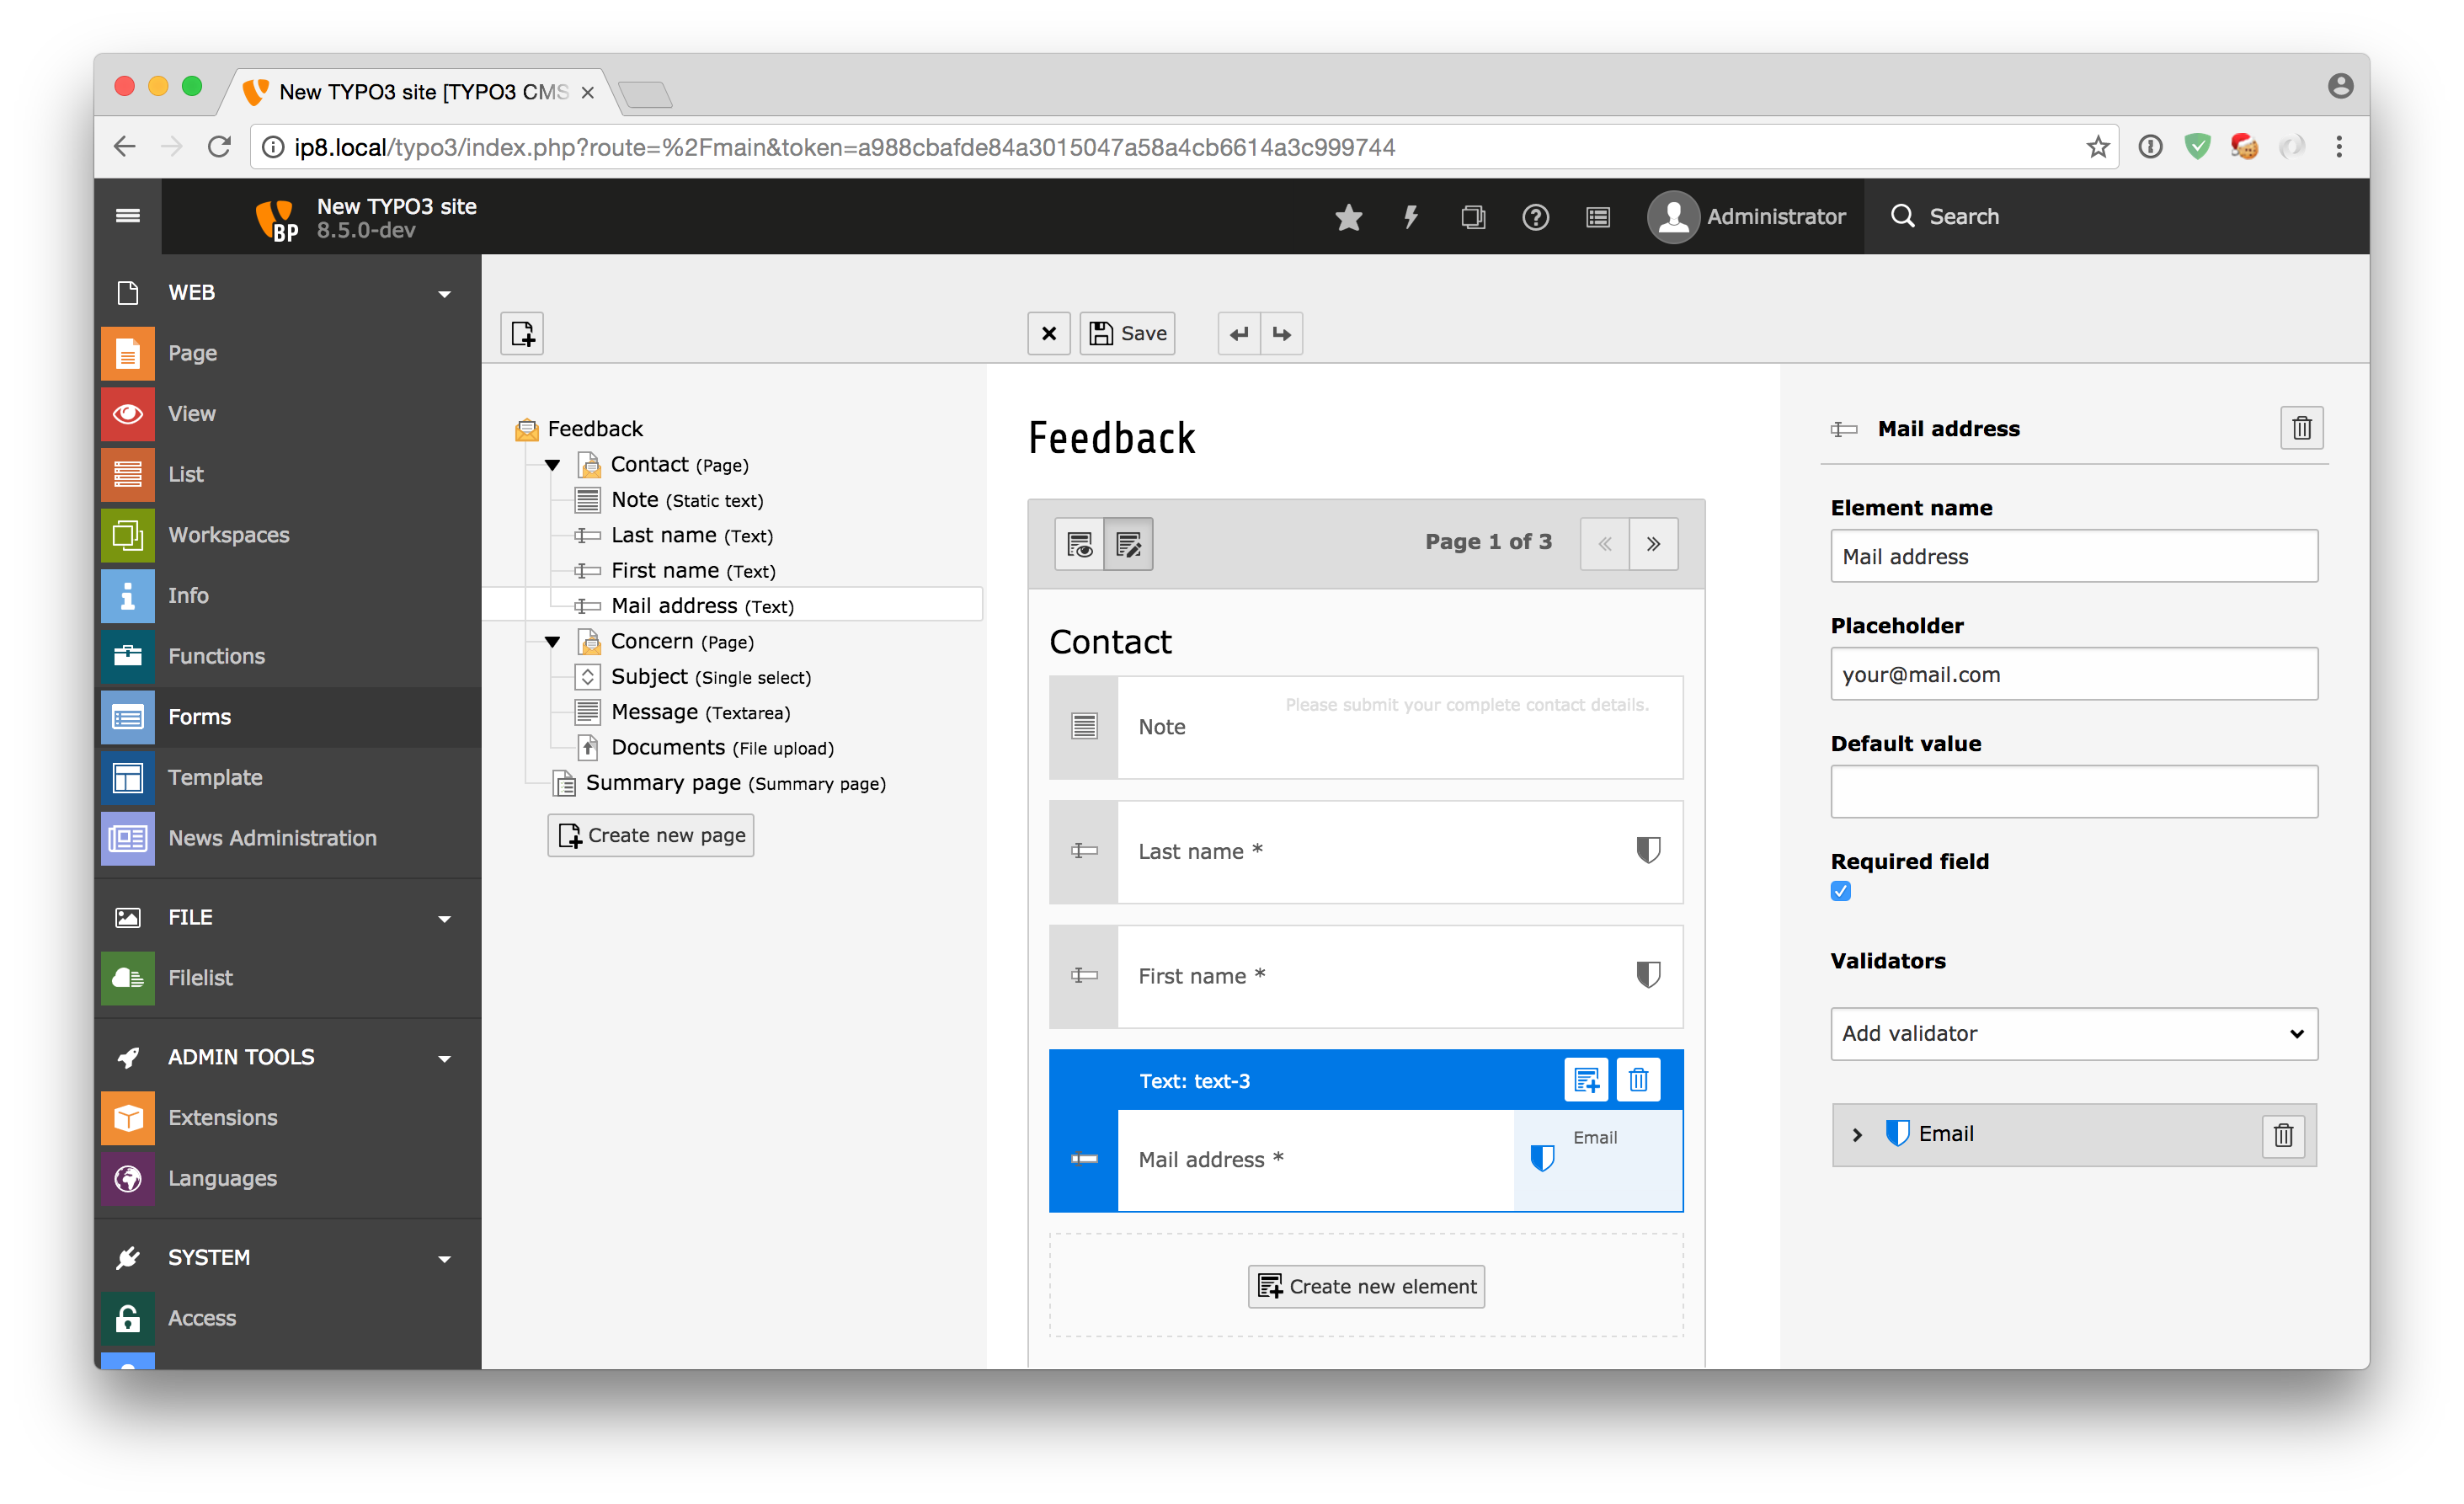
\includegraphics[width=0.8\linewidth]{FormFramework/form-framework-1.png}
	\end{figure}

\end{frame}

% ------------------------------------------------------------------------------
% LTXE-SLIDE-START
% LTXE-SLIDE-UID:		a93f3357-6a22f111-1dac29b0-bedf5bf0
% LTXE-SLIDE-ORIGIN:	b91ec75b-7aa7b566-b523ca5f-f9ba3cde English
% LTXE-SLIDE-TITLE:		#77910: New Form Framework (4)
% ------------------------------------------------------------------------------
\begin{frame}[fragile]
	\frametitle{Gebruikersinterface backend}
	\framesubtitle{Screenshot (2)}

	\begin{figure}
		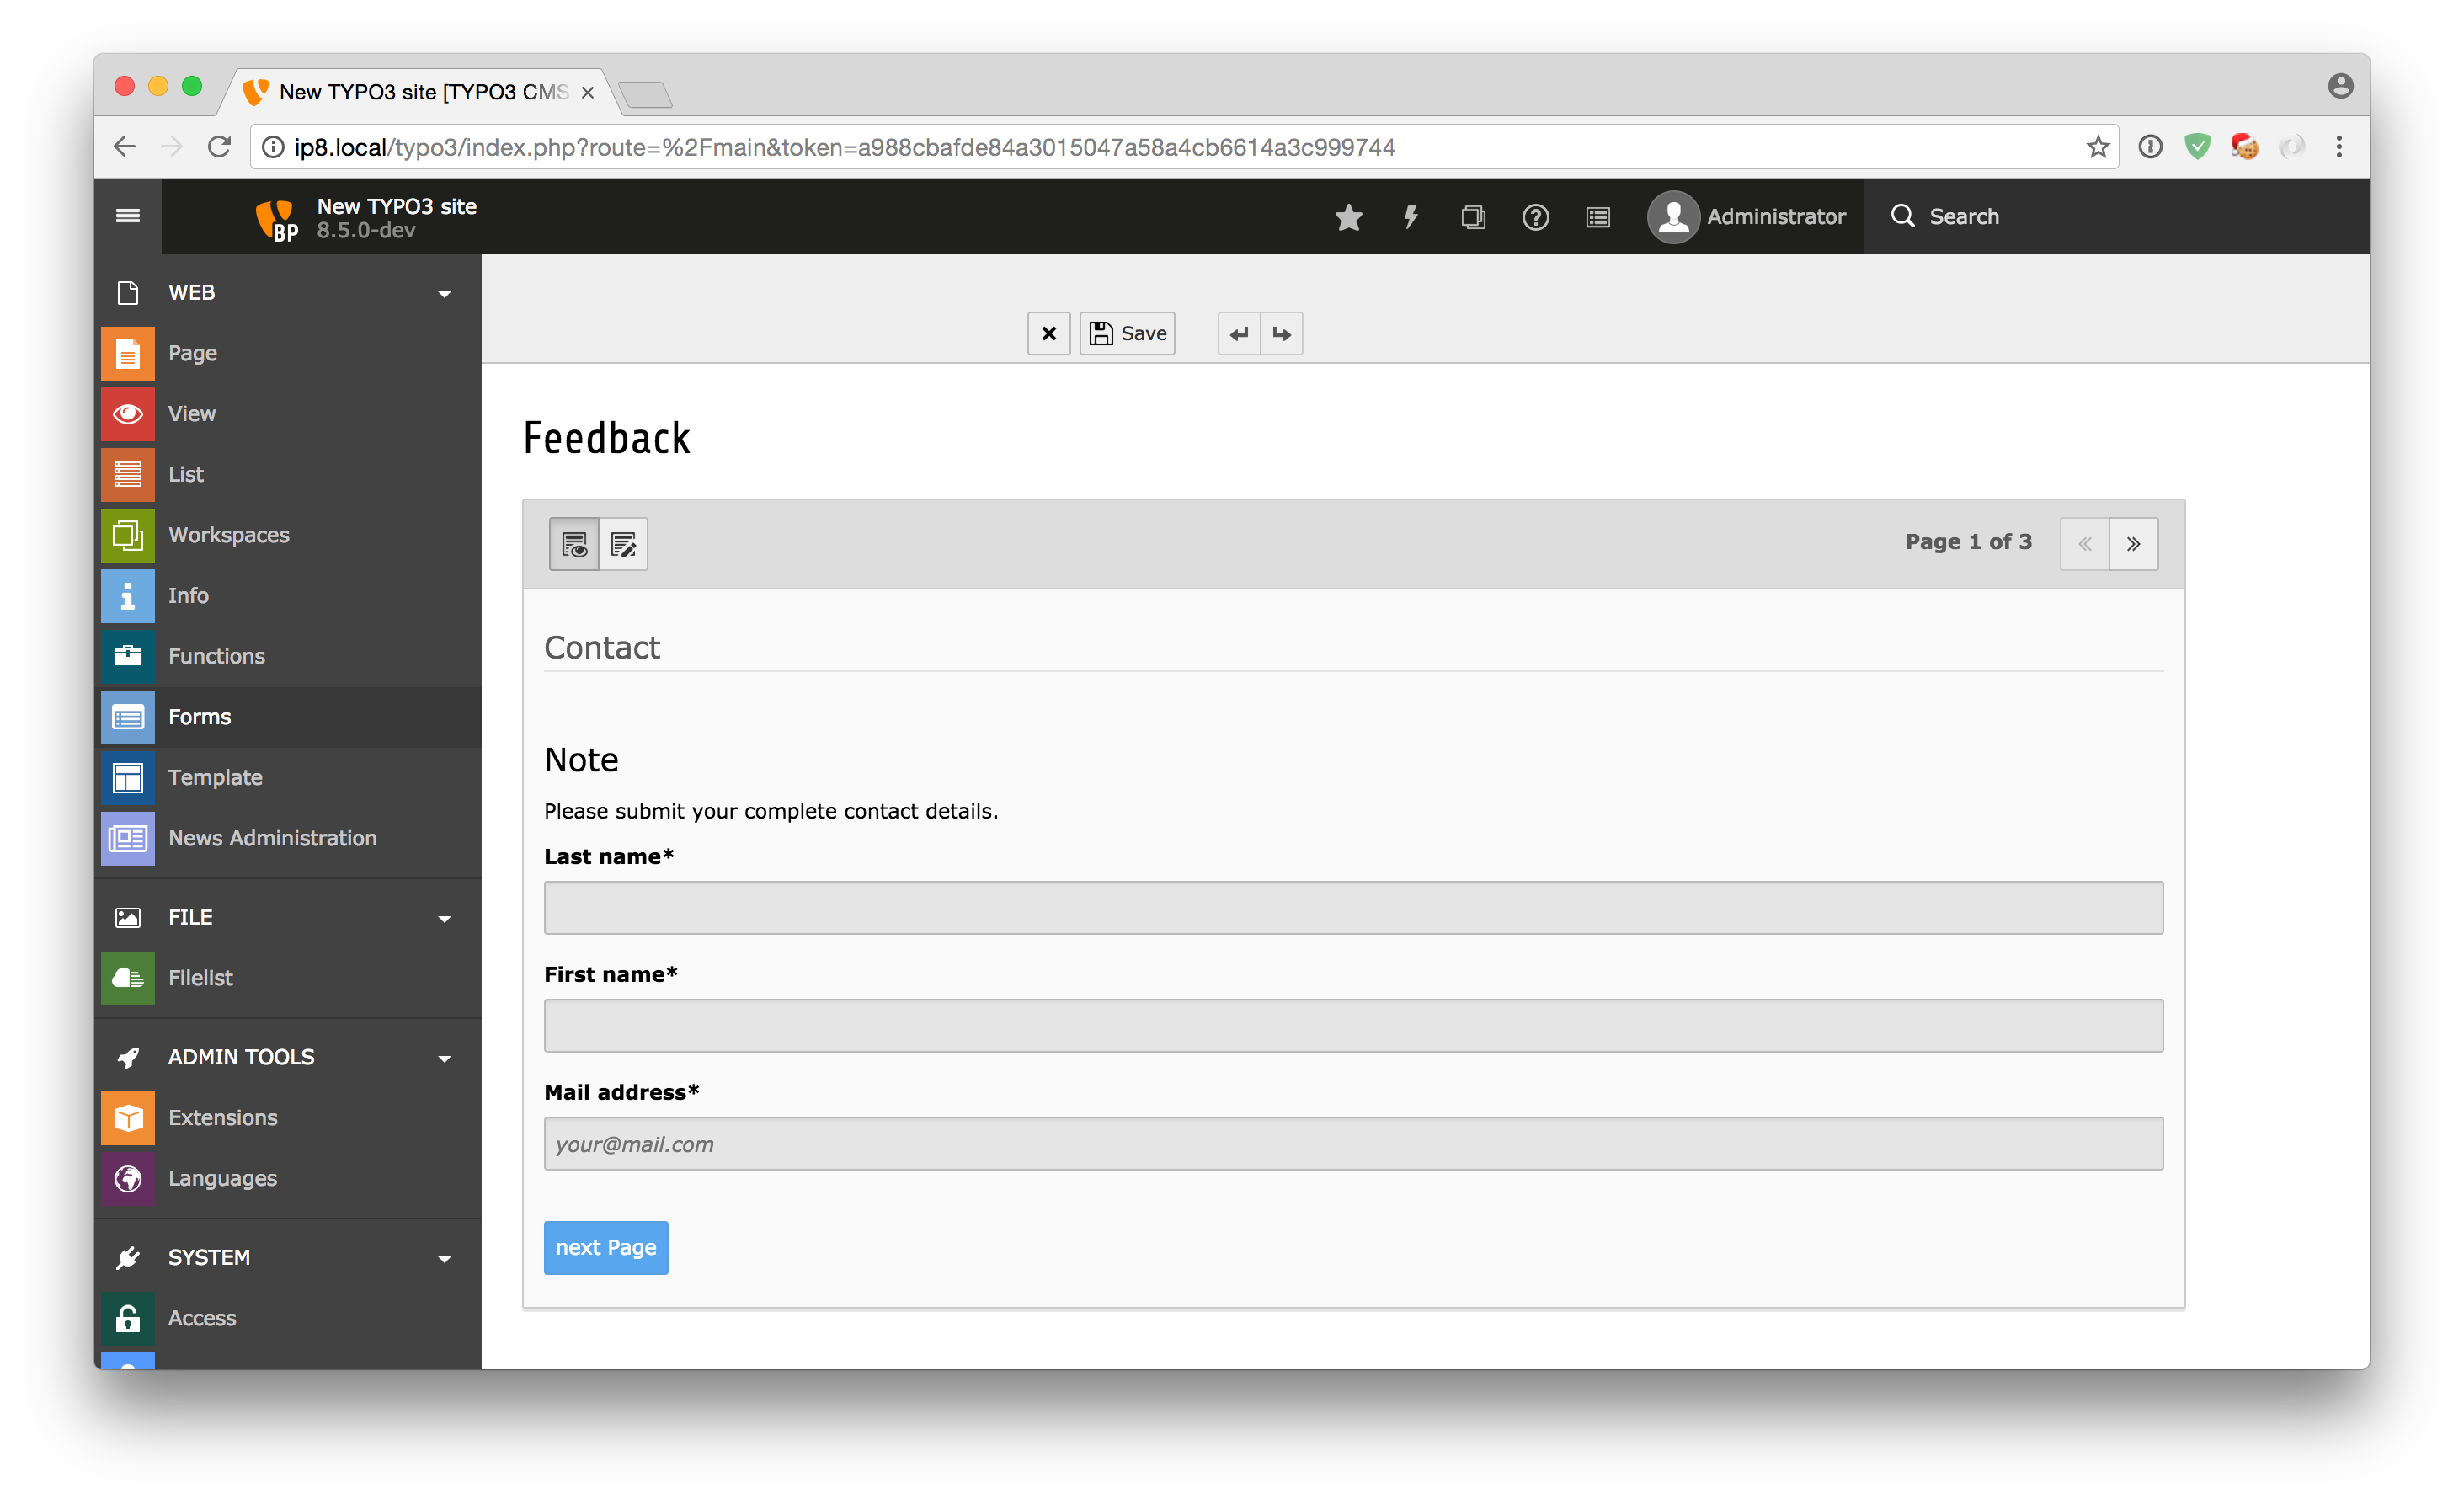
\includegraphics[width=0.8\linewidth]{FormFramework/form-framework-2.png}
	\end{figure}

\end{frame}

% ------------------------------------------------------------------------------
